\documentclass[10pt,a4paper]{article}

\usepackage[utf8]{inputenc}
\usepackage[T1]{fontenc}
\usepackage[italian]{babel}
\usepackage{graphicx}
\usepackage{amsmath,amssymb,amsfonts}
\usepackage{caption}
\usepackage{subcaption}
\usepackage{wrapfig}
\usepackage{float}
\usepackage{geometry}
\geometry{top=2.5cm, bottom=2.5cm, left=1.7cm, right=1.7cm}
\usepackage{fancyhdr}
\usepackage{titlesec}
\usepackage{lmodern}
\usepackage{caption}
\usepackage{comment}
\usepackage{booktabs}
\usepackage{makecell}
\usepackage{siunitx}
\usepackage[version=4]{mhchem} 
\DeclareCaptionFont{myit}{\footnotesize\itshape\fontfamily{cmr}\selectfont}
\captionsetup{
    font=myit,
    labelfont={bf},
    textfont=normalfont
}
\usepackage{titletoc}

% Intestazioni moderne
\pagestyle{fancy}
\fancyhf{}
\fancyhead[L]{Vita media del $\mu$}
\fancyhead[R]{Niccolò Menichetti \\ Luca Musetti \\ Luca Nasone}
\fancyfoot[C]{\thepage}

% Re e Im
\renewcommand{\Re}{\mathop{\mathrm{Re}}}
\renewcommand{\Im}{\mathop{\mathrm{Im}}}

% Per "simulare" capitoli
\newcommand{\chapter}[1]{
    \clearpage
    \section*{#1}
    \addcontentsline{toc}{section}{#1}
}

\title{\bfseries Relazione di laboratorio \\[1ex] \Large Vita media del $\mu$}
\author{Niccolò Menichetti \\ Luca Musetti \\ Luca Nasone}
\date{Anno Accademico 2025--2026}

\begin{document}

\begin{titlepage}
    \thispagestyle{empty}
    
    \begin{figure}[ht]
        \centering
        \begin{minipage}{0.48\textwidth}
            \centering
            
\includegraphics[width=5.0cm]{Stemma_unipi.svg.png}
        \end{minipage}%
        \hfill
        \begin{minipage}{0.48\textwidth}
            \centering
            
\includegraphics[width=7.0cm]{unipi_fermi.png}
        \end{minipage}
    \end{figure}

    \vspace{4.0cm} % Spazio per centrare verticalmente il contenuto

    \begin{center}
        {\fontsize{20pt}{24pt}\selectfont\bfseries Vita media del muone}\\[0.3cm]
        {\large Relazione laboratorio di interazioni fondamentali}\\[9.0cm]

        {\Large NICCOLO' MENICHETTI\hspace{0.2cm} LUCA MUSETTI \hspace{0.2cm} LUCA NASONE}\\[0.35cm]
        {\normalsize Anno Accademico 2025 - 2026}
    \end{center}

\end{titlepage}

\newpage

\begin{abstract}
        
    \emph{Nella seguente relazione descriviamo la nostra misura della vita media del muone, effettuata sui muoni dei raggi cosmici. Otteniamo una vita media pari a ...(To be continued...)}
        
\end{abstract}

\tableofcontents

\newpage

\section{Introduzione}

A livello del mare, a causa dell'interazione con l'atmosfera, i raggi cosmici sono principalmente costituiti da muoni $\mu$, una particella instabile che decade nel seguente modo:

\begin{center}
    \ce{$\mu^{-}\rightarrow e^{-}\bar \nu_e \nu_{\mu}$}
\end{center}

con vita media è $\tau_{\mu} = 2.1969811 \pm 0.0000022 $ $\mu s$ (PDG 2025) e carica $\pm e$.

L'obiettivo dell'esperimento è misurare il valore della vita media  di questa particella, con un apparato sperimentale in grado di rilevare i raggi cosmici e fermare i $\mu$ a bassa energia. Dai dati ottenuti è stato inoltre possibile stimare l'abbondanza relativa di $\mu^{+}$ e $\mu^{-}$. 

Con opportune modifiche è stato possibile misurare lo spettro in energia dell'$e^{-}$ del decadimento. Siccome lo spettro è limitato superiormente da:
\begin{center}
    $(E_e)^{max} = \frac{m_{\mu}^2+m_{e}^2}{2m_{\mu}}$
\end{center}
da quest'ultima misura sarà possibile ottenere una stima della massa del $\mu$.

\section{Apparato sperimentale}

\begin{figure}[h]
\centering
\begin{minipage}{0.45\textwidth}
    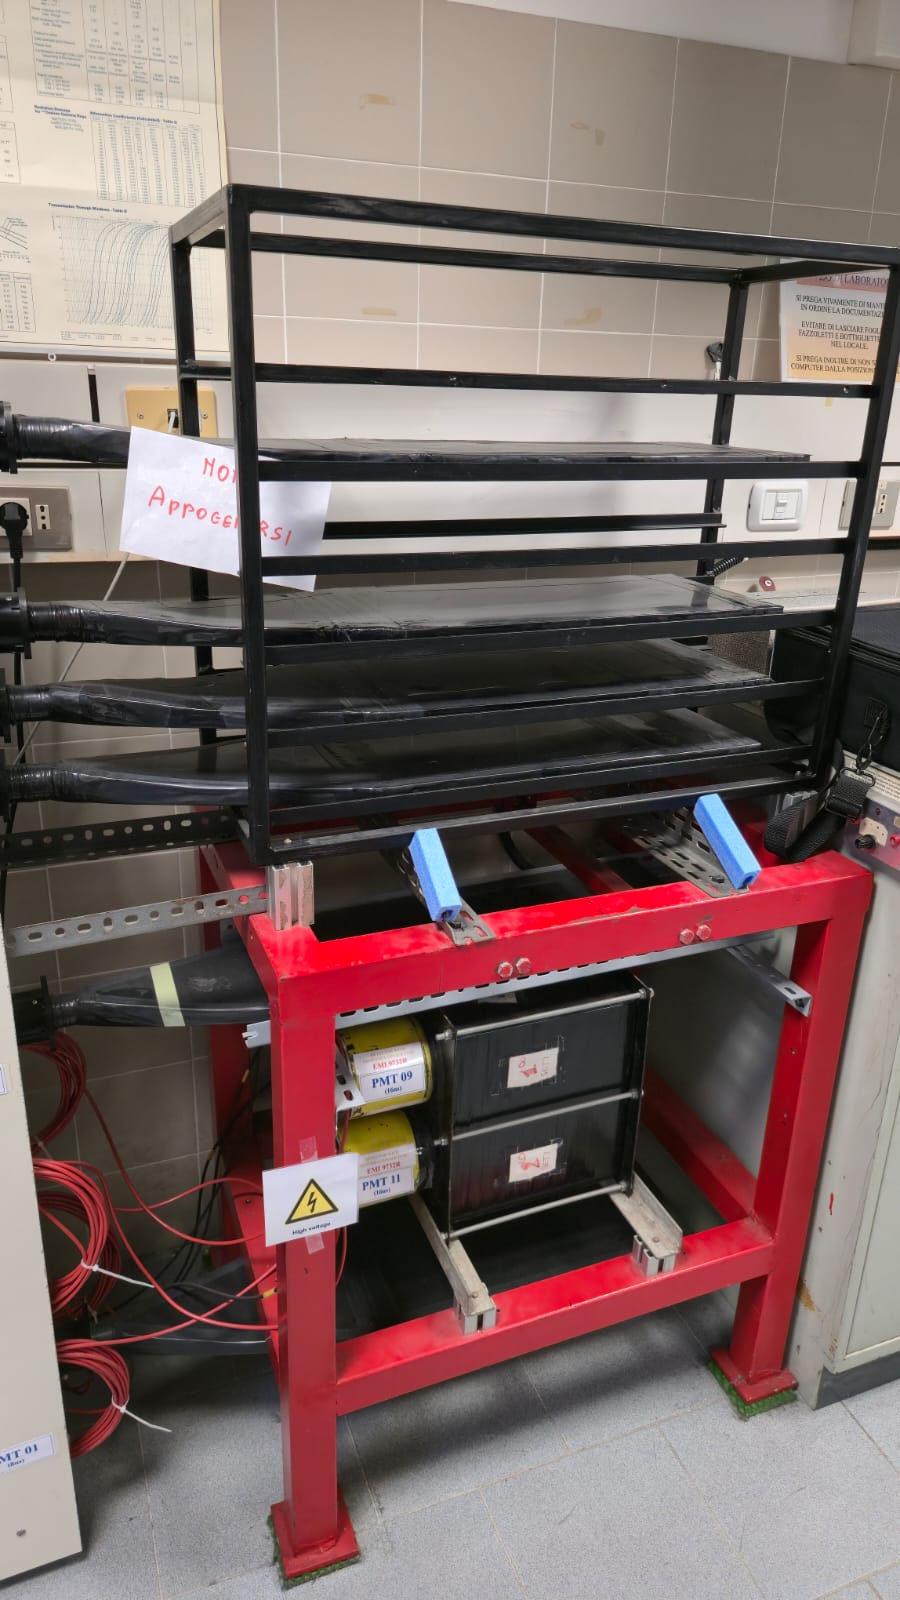
\includegraphics[width=0.55\linewidth]{WhatsApp Image 2025-12-06 at 15.04.09 (3).jpeg}
    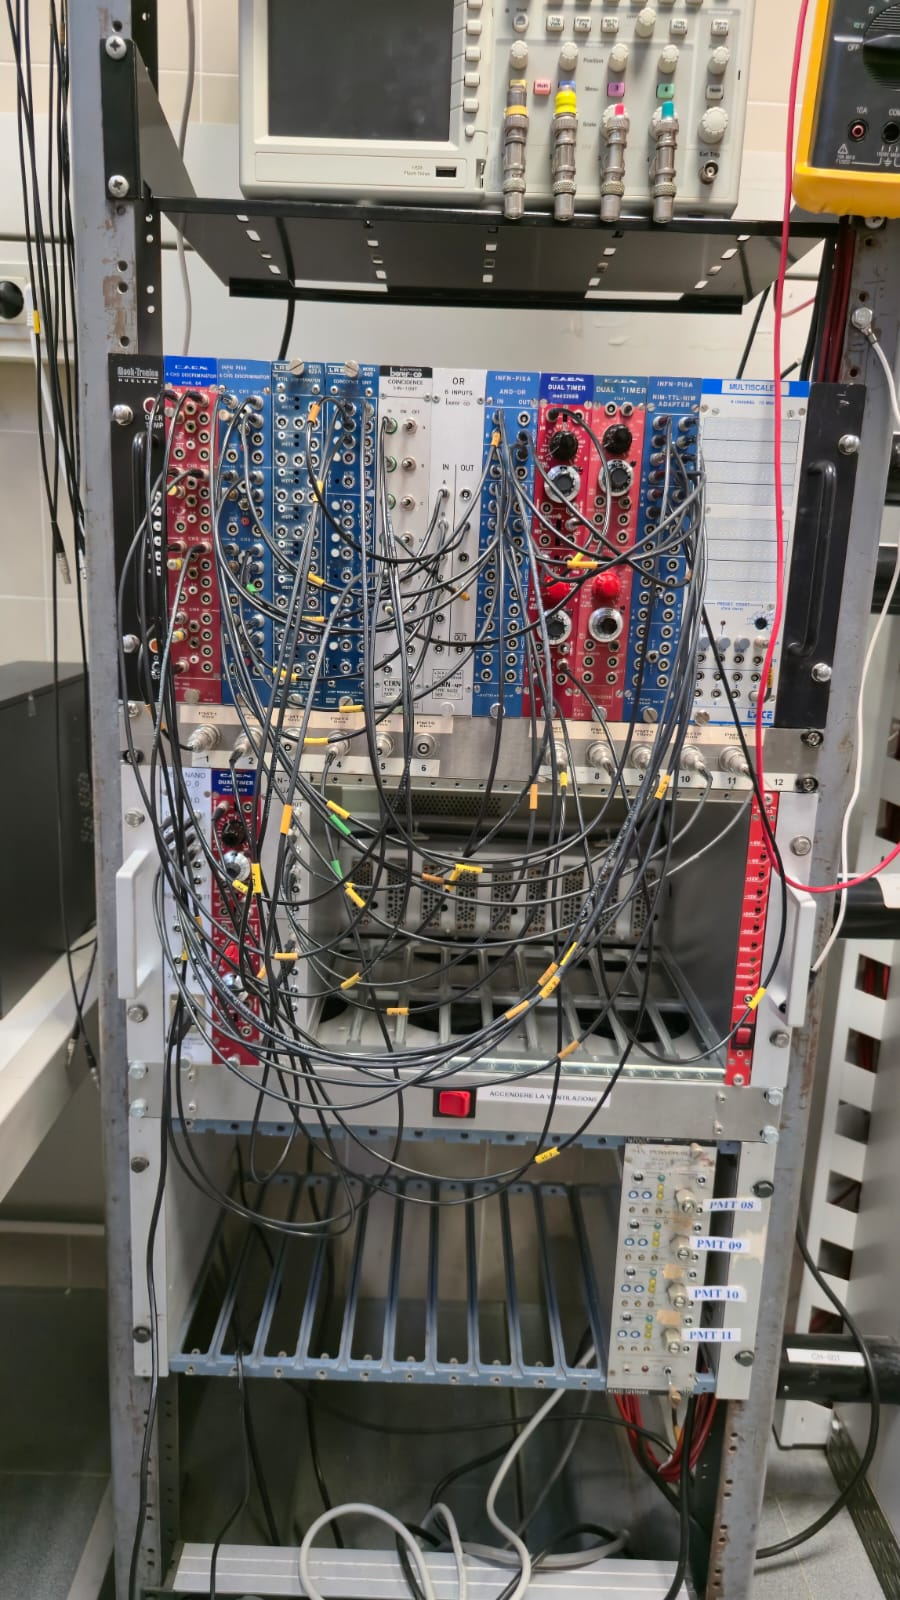
\includegraphics[width=0.55\linewidth]{WhatsApp Image 2025-12-06 at 15.04.09 (2).jpeg}
\end{minipage}
\begin{minipage}{0.45\textwidth}
    \begin{itemize}
    \item 6 lastre di scintillatore lette ciascuno da un fotomoltiplicatore (PMT);
    \item 1 blocco di scintillatore letto da 4 PMT;
    \item una scheda DE0-10 NANO;
    \item 2 discriminatori (NIM CAEN N84 e NIM INFN);
    \item 3 unità di coincidenza (NIM LRS 465, NIM CERN N6234, NIM);
    \item 1 unità di OR (NIM CERN);
    \item 2 unità di Dual Timer (NIM CAEN mod2255B e NIM CAEN N2255);
    \item 1 unità di conversione NIM-TTL;
    \item 1 multiscaler (NIM INFN Multiscaler130);
    \item 1 unità di Fan-Out;
    \item 1 integratore analogico (NIM CAEN N914);
    \item 1 ADC (NIM CAEN N6725);
    \item 1 oscilloscopio;
    \item 2 computer, per regolare le alimentazioni e per le acquisizioni;
    \item 1 multimetro;
    \item cavi coassiali di vario ritardo e terminazioni a 50 e 0 $\Omega$;
    \item 1 metro a nastro;
\end{itemize}
\end{minipage}
\end{figure}


\newpage

\section{Caratterizzazione dell'apparato}

\subsection{Telescopio}

La prima attività svolta in laboratorio è stato scegliere il punto di lavoro dei vari PMT. Soglie e alimentazioni influenzano l'efficienza e di conseguenza il numero di eventi rivelati. Vogliamo sia più alta possibile. 

Sono stati scelti il PMT07, il PMT04 e il PMT02. Stimiamo l'efficienza di un PMT con il rapporto fra le coincidenze triple e le coincidenze doppie degli altri due. Tali conteggi sono misurati mandando i segnali discriminati prima alle unità di coincidenza e in seguito al multiscaler, per 100 s. La misura viene poi ripetuta variando l'alimentazione.

Durante la procedura sono state misurate anche le singole degli altri due PMT, in quanto il rate in singola influenza il rate delle doppie fake, ottenuto da:

\begin{center}

    $ R_{fake} = R_1 R_2 (w_1 + w_2 - 2w)$

\end{center}

Dove $R_1$ e $R_2$ sono i rate in singola dei PMT usati per calcolare le doppie, $w_1$ e $w_2$ sono le durate dei loro segnali discriminati (50 ns nel nostro caso). $w$ è la sovrapposizione temporale minima per avere una coincidenza, di 2 ns. Sceglieremo alimentazioni e soglie cercando di rendere il numero di doppie fake trascurabile rispetto alle doppie misurate.

Tale procedura è ottimale per il PMT mediano (il PMT04), ma non per il PMT07 e PMT02, in quanto sottostima l'efficienza a causa della geometria del sistema. Per correggere tale effetto abbiamo simulato il sistema con un Montecarlo in modo da ricavare la probabilità che un raggio cosmico passi per un PMT dato il passaggio dagli altri due (accettanza). Dividendo il rapporto triple su doppie con tale valore si ottiene una stima più accurata dell'efficienza.

Come errore sull'efficienza riportiamo : 

\begin{center}

    $ \sigma_{\varepsilon} = \sqrt{\frac{\varepsilon(1-\varepsilon)}{D}}$
  
\end{center}

Con $D$ il numero di doppie.

Riportiamo di seguito le curve di efficienza : 

\begin{figure}[h]
\centering

\includegraphics[width = 0.7\textwidth]{Efficiency Curves - Telescope.png}
\caption{Grafico delle curve di efficenza per i PMT02, -04, -07}
\end{figure}

Riportiamo inoltre le misure effettuate in tabella:

\newpage

\centering

\textbf{PMT02}

\vspace{0.25cm}

\begin{tabular}{|c|c|c|c|}
\toprule
$HV$[kV]& $\varepsilon$ [$\%$] & $\sigma_{\varepsilon}$[$\%$] & $D_{fake}$ [pure] \\
\midrule
1.675 & 52 & 2 & 0.69 \\
1.700 & 70 & 2 & 0.65 \\
1.720 & 80 & 1 & 0.63 \\
1.730 & 81 & 1 & 0.59 \\
1.750 & 89 & 1 & 0.53 \\
1.775 & 80 & 1 & 0.54 \\
1.800 & 91 & 1 & 0.56 \\
\bottomrule
\end{tabular}

\vspace{1cm}

\textbf{PMT04}

\vspace{0.25cm}

\begin{tabular}{|c|c|c|c|}
\toprule
$HV$[kV]& $\varepsilon$ [$\%$] & $\sigma_{\varepsilon}$[$\%$] & $D_{fake}$ [pure] \\
\midrule
1.675 & 87 & 2 & 0.077 \\
1.700 & 94 & 1 & 0.068 \\
1.720 & 94 & 1 & 0.074 \\
1.730 & 92 & 2 & 0.073 \\
1.750 & 93 & 1 & 0.078 \\
1.775 & 94 & 1 & 0.076 \\
1.800 & 92 & 1 & 0.076 \\
\bottomrule
\end{tabular}

\vspace{1cm}

\textbf{PMT07}

\vspace{0.25cm}

\begin{tabular}{|c|c|c|c|}
\toprule
$HV$[kV]& $\varepsilon$ [$\%$] & $\sigma_{\varepsilon}$[$\%$] & $D_{fake}$ [pure] \\
\midrule
1.675 & 50 & 2 & 0.97 \\
1.700 & 77 & 2 & 0.79 \\
1.720 & 83 & 1 & 0.73 \\
1.730 & 78 & 2 & 0.73 \\
1.750 & 80 & 2 & 0.68 \\
1.775 & 92 & 1 & 0.64 \\
1.800 & 88 & 1 & 0.57 \\
\bottomrule
\end{tabular}

\vspace{1cm}

In conclusione il punto di lavoro scelto per il telescopio è:

\vspace{1cm}

\begin{tabular}{|c|c|c|c|}
\toprule
Parametro & PMT02 & PMT04 & PMT07 \\
\midrule
$V_{supply}$ [kV] & 1.750 & 1.700 & 1.750  \\
$V_{thr}$ [mV] & -30 & -30 & -30  \\
$\varepsilon$ [$\%$] & 88 & 94 & 79 \\
\bottomrule
\end{tabular}

\subsection{Blocco}

\subsection{VETO}

\end{document}